\documentclass[mathserif,serif]{beamer}
\usepackage{pdfpages} 
\usepackage{graphics}
\definecolor{WinterSkin}{HTML}{E9E9EA}
\usepackage{amsmath,amssymb,amsfonts,textcomp,setspace,graphicx,lipsum,hanging,url}
\setbeamercolor{frametitle}{fg=black}
\setbeamercolor{background canvas}{bg=white}
\begin{document}
  \begin{frame}
    \frametitle{\centerline{NFL Go For It!}\\
\bigskip
 \centerline{\LARGE The 4th Down Decision}}
    %Frame 1
\begin{figure}
\begin{center}
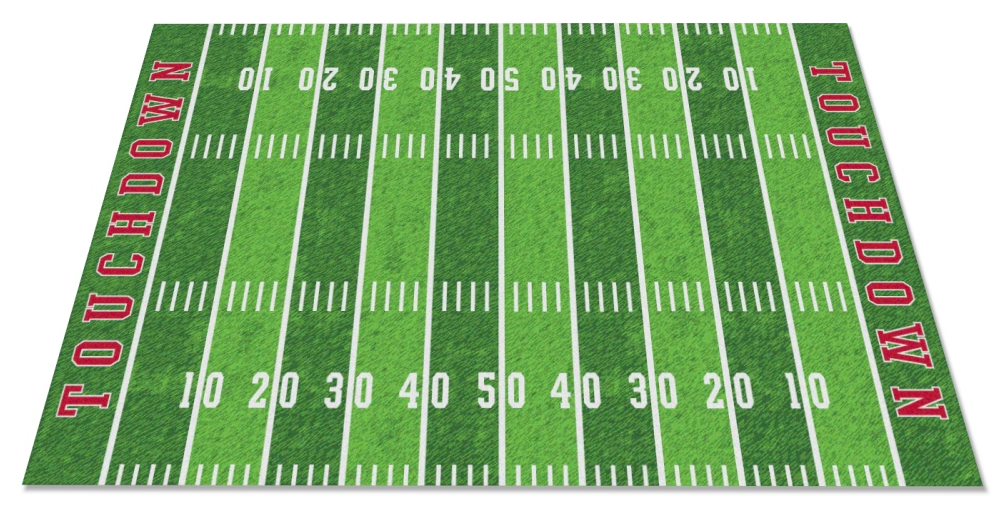
\includegraphics[width=1\textwidth]{FootballField.png}
\end{center}
\end{figure}
\begin{center}
\large by Mike Ghirardo and Thomas McCann
\end{center}
  \end{frame}
\begin{frame}
 \frametitle{\centerline{NFL Go For It!}}
In American Football there are many decisions a team needs to make in order to win the game. In this project we focus on those that need to be made on 4th down plays. Following are the three decisions to be made on the fourth down. \\
\begin{enumerate}[1.]
\item 
Punt
\item
Kick a field goal
\item
Go for a first down
\end{enumerate}
\end{frame}
\begin{frame}
 \frametitle{\centerline{NFL Go For It!}}
We attempt to determine which choice should be made under certain conditions. The following are the conditions which we take into account in determining the best action.
\begin{enumerate}[1.]
\item
Offensive and defensive rank of the offensive team
\item
Offensive and defensive rank of the defensive team
\item
The number of yards to convert a first down
\item
The field position
\end{enumerate}
With this information from the data we were able to estimate the expected points scored given each of the three decisions.\\
Finally, with this information a decision can be made.
\end{frame}
  \begin{frame}
    \frametitle{\centerline{NFL Go For It!}}
    %Frame 2
\centerline{\Large The Data}
\bigskip
The data that we have chosen to attempt to answer this research question is NFL play-by-play data for seasons 2002 - 2012. The play-by-play data includes a game ID, which quarter, which down, which teams, a play description, and the number of points scored.
  \end{frame}
 \begin{frame}
    \frametitle{\centerline{NFL Go For It!}}
\centerline{\Large Determining the Decision}
\bigskip
Let $Points_{o}$ and $Points_{d}$ be the number of points the offensive and defensive team will score respectively. Let $Punt$, $Field Goal$, and $Go For It$ be the events that the offensive team punts, attempts a field goal and goes for the 1st down given they are on their fourth down respectively. Let $S_{f}$ and $S_{g}$ be the events that the offensive team successfully scores a field goal and successfully converts a first down respectively. Then let
{\footnotesize
\begin{gather*}
P = E[Points_{o} | Punt] \\
G = E[Points_{o}|Go For It] = E[Points_{o}| S_{g}]P(S_{g}) - E[Points_{d}|S_{g}^c]P(S_{g}^c)\\
F = E[Points_{o}|Field Goal] = E[Points_{o}| S_{f}]P(S_{f}) - E[Points_{d}|S_{f}^c]P(S_{f}^c)\\
\end{gather*}
}%
Then Decision $= argmax\{P, G, F\}$.
  \end{frame}
%  \begin{frame}
%    \frametitle{\centerline{NFL Go For It!}}
%\begin{center}
%\end{center}
%\begin{figure}
%\begin{center}
%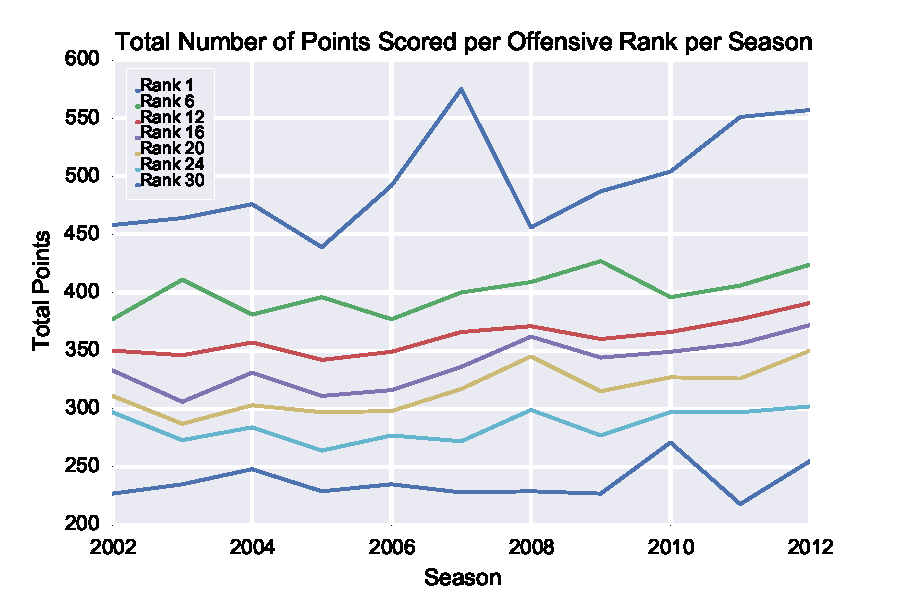
\includegraphics[width=1\textwidth]{OffRankperSeason.pdf}
%\end{center}
%\end{figure}
%  \end{frame}
%  \begin{frame}
 %   \frametitle{\centerline{NFL Go For It!}}
%\begin{center}
%\end{center}
%\begin{figure}
%\begin{center}
%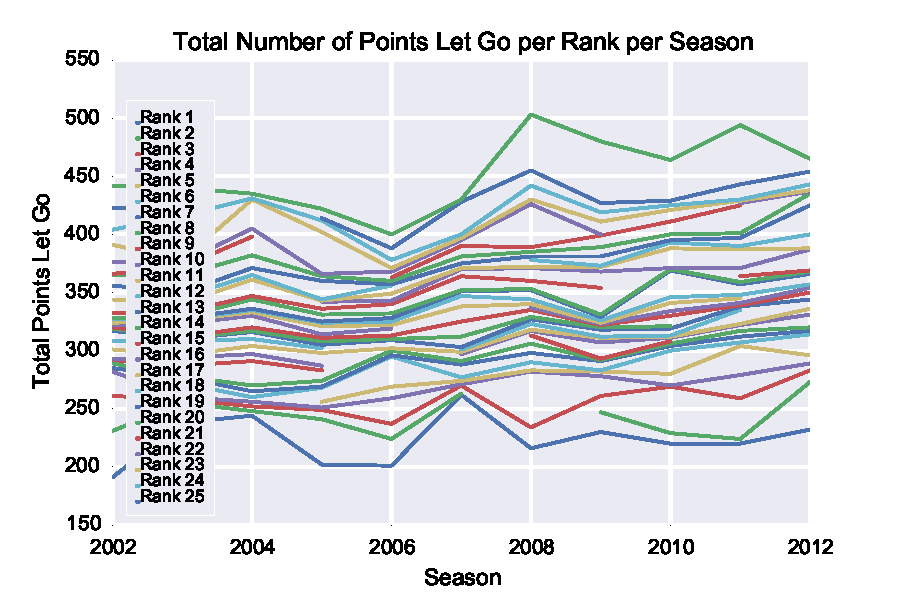
\includegraphics[width=1\textwidth]{DefRankperSeason.pdf}
%\end{center}
%\end{figure}
%  \end{frame}
  \begin{frame}
    \frametitle{\centerline{NFL Go For It!}}
\begin{center}
\end{center}
\begin{figure}
\begin{center}
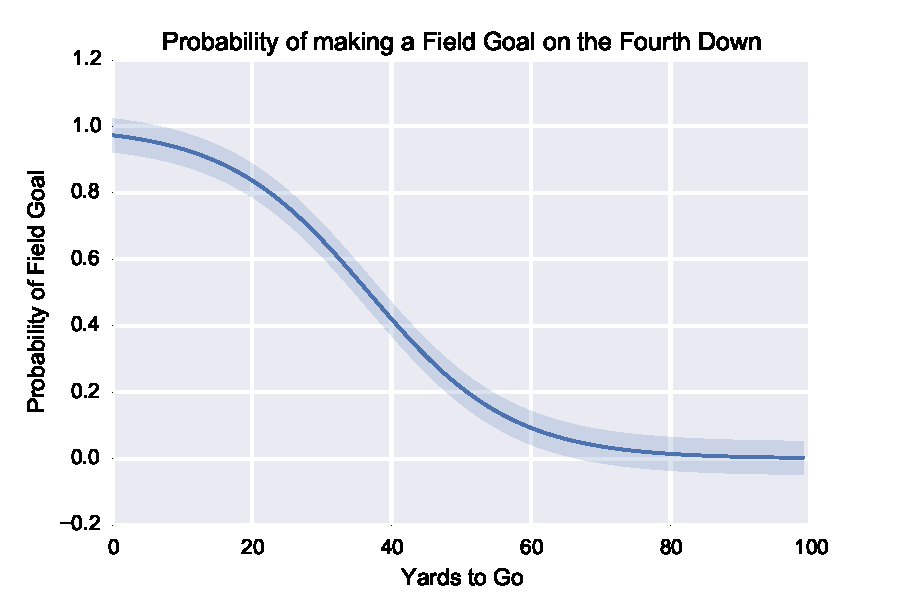
\includegraphics[width=1\textwidth]{fieldgoalprob.pdf}
\end{center}
\end{figure}
  \end{frame}
%\begin{frame}
%\frametitle{\centerline{NFL Go For It!}}
%\begin{figure}
%\begin{center}
%\includegraphics[width=1\textwidth]{z1plot.pdf}
%\end{center}
%\end{figure}
%  \end{frame}
  \begin{frame}
    \frametitle{\centerline{NFL Go For It!}}
\begin{figure}
\begin{center}
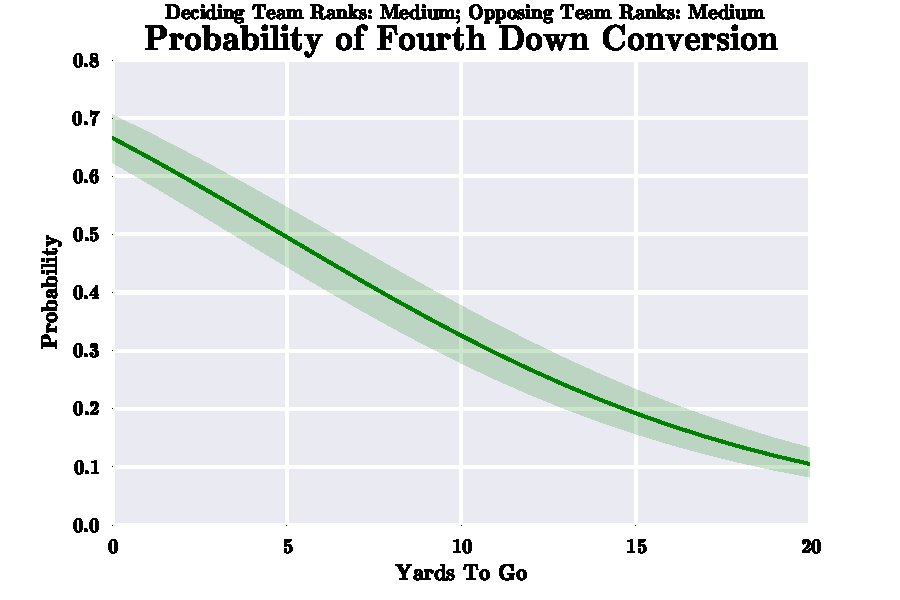
\includegraphics[width=1\textwidth]{gfi_15_15_prob.pdf}
\end{center}
\end{figure}
  \end{frame}
%  \begin{frame}
%    \frametitle{\centerline{NFL Go For It!}}
%\begin{figure}
%\begin{center}
%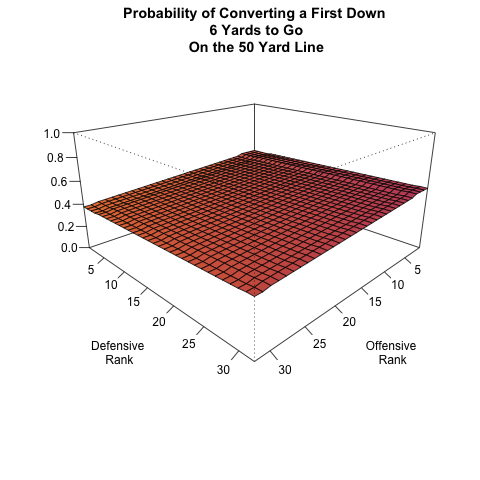
\includegraphics[width=1\textwidth]{z3plot.png}
%\end{center}
%\end{figure}
%  \end{frame}
% \begin{frame}
%   \frametitle{\centerline{NFL Go For It!}}
%\begin{figure}
%\begin{center}
%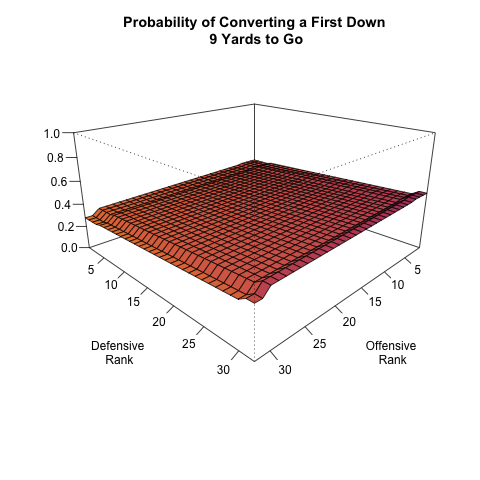
\includegraphics[width=1\textwidth]{z4plot.png}
%\end{center}
%\end{figure}
%  \end{frame}
  \begin{frame}
    \frametitle{\centerline{NFL Go For It!}}
\begin{figure}
\begin{center}
%Offense Rank: Medium; Defense Rank: Medium
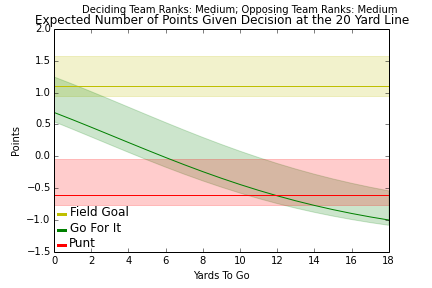
\includegraphics[width=1\textwidth]{Decision2015161516.png}
\end{center}
\end{figure}
  \end{frame}
\begin{frame}
    \frametitle{\centerline{NFL Go For It!}}
\begin{figure}
\begin{center}
%Offense Rank: Medium; Defense Rank: Medium
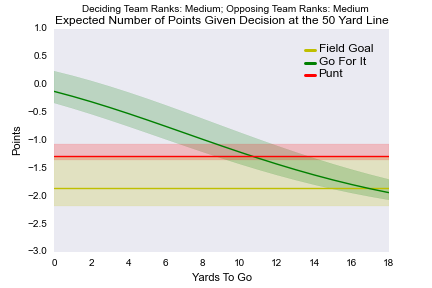
\includegraphics[width=1\textwidth]{Decision5015161516.png}
\end{center}
\end{figure}
  \end{frame}
  \begin{frame}
   \frametitle{\centerline{NFL Go For It!}}
\begin{figure}
\begin{center}
%Offense Rank: Medium; Defense Rank: Medium
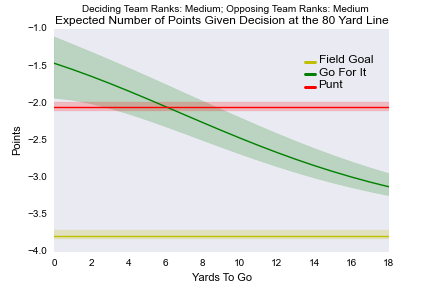
\includegraphics[width=1\textwidth]{Decision8015161516.png}
\end{center}
\end{figure}
  \end{frame}
 \begin{frame}
    \frametitle{\centerline{NFL Go For It!}}
\centerline{\LARGE Determining the Decision}
\begin{center}
50 Yard Line, 5 Yards to Go \\
Offense Rank: Medium; Defense Rank: Medium \\
\end{center} 
{\footnotesize
\begin{gather*}
P = E[Points_{o} | Punt] = -1.28 \\
G = E[Points_{o}|Go For It] = E[Points_{o}| S_{g}]P(S_{g}) - E[Points_{d}|S_{g}^c]P(S_{g}^c)\\
    = 1.29(.50) + (-2.52)(1 - .50) = -.63 \\
F = E[Points_{o}|Field Goal] = E[Points_{o}| S_{f}]P(S_{f}) - E[Points_{d}|S_{f}^c]P(S_{f}^c)\\
   = 1.63(.21) + (-2.80)(1 - .21) = -1.86 \\
\end{gather*}
\centerline{\large Decision $= argmax\{P, G, F\}$} \\
\bigskip
\centerline{\large $= argmax\{-1.28, -0.63, -1.86\} = $ Go For It!.}
}%
  \end{frame}
 \begin{frame}
   \frametitle{\centerline{NFL Go For It!}\\ \centerline{What should my decision be?}}
\begin{figure}
\begin{center}
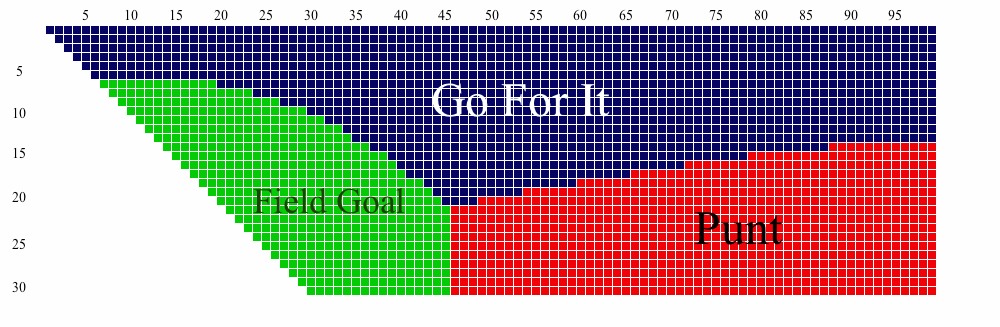
\includegraphics[width=1\textwidth]{GridBlock112525.png}
\end{center}
\end{figure}
  \end{frame}
\begin{frame}
    \frametitle{\centerline{NFL Go For It!}\\ \centerline{What should my decision be?}}
\begin{figure}
\begin{center}
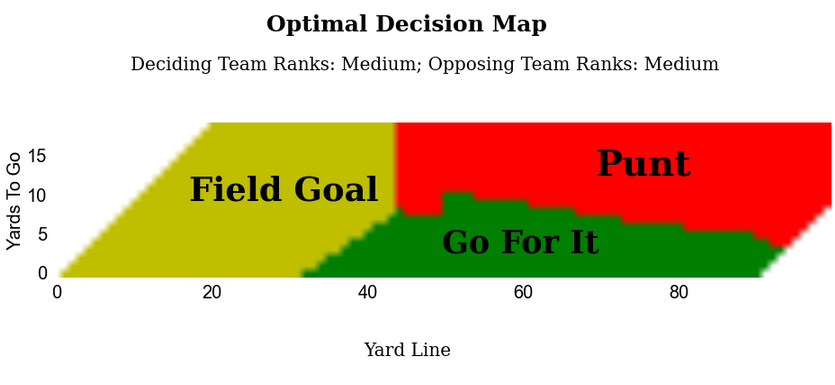
\includegraphics[width=1\textwidth]{GridBlock15151515.png}
\end{center}
\end{figure}
  \end{frame}
\begin{frame}
    \frametitle{\centerline{NFL Go For It!}\\ \centerline{What should my decision be?}}
\begin{figure}
\begin{center}
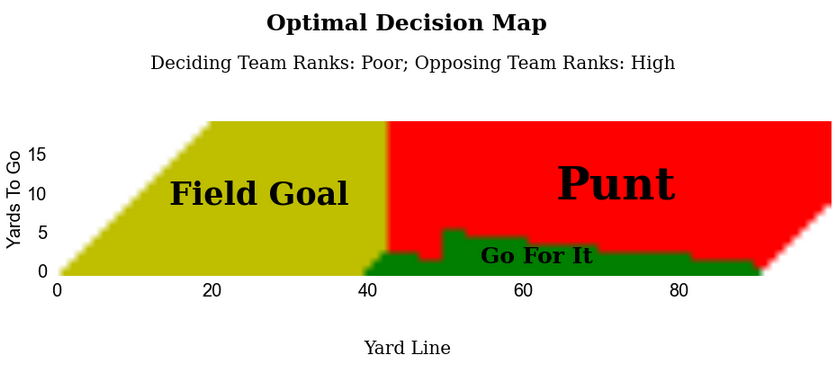
\includegraphics[width=1\textwidth]{GridBlock252511.png}
\end{center}
\end{figure}
 \end{frame}
\setbeamerfont{LargeFont}{size=\Large}
\begin{frame}
\usebeamerfont{LargeFont}
\begin{center}
\Large{Thank You!}
\end{center}
  \end{frame}
\end{document}